\begin{figure}
\centering
      \begin{subfigure}[b]{0.3\textwidth}
          \centering
          
\includegraphics[width=\textwidth]{Figures/giqlogo.png}
          \caption{x = y}
      \end{subfigure}
      \hfill
      \begin{subfigure}[b]{0.3\textwidth}
          \centering
          
\includegraphics[width=\textwidth]{Figures/giqlogo.png}
          \caption{x = y}
      \end{subfigure}
      \hfill
      \begin{subfigure}[b]{0.3\textwidth}
          \centering
          
\includegraphics[width=\textwidth]{Figures/giqlogo.png}
          \caption{x = y}
      \end{subfigure}
\caption{this is the big caption}
\end{figure}

\begin{figure}
    \centering
    
\includegraphics[width=0.5\textwidth]{Figures/giqlogo.png}
    \caption{Caption}
    \label{fig:my_label}
\end{figure}







\begin{figure}[t!]
    \centering
    \begin{subfigure}[b]{0.49\textwidth}
        \centering
        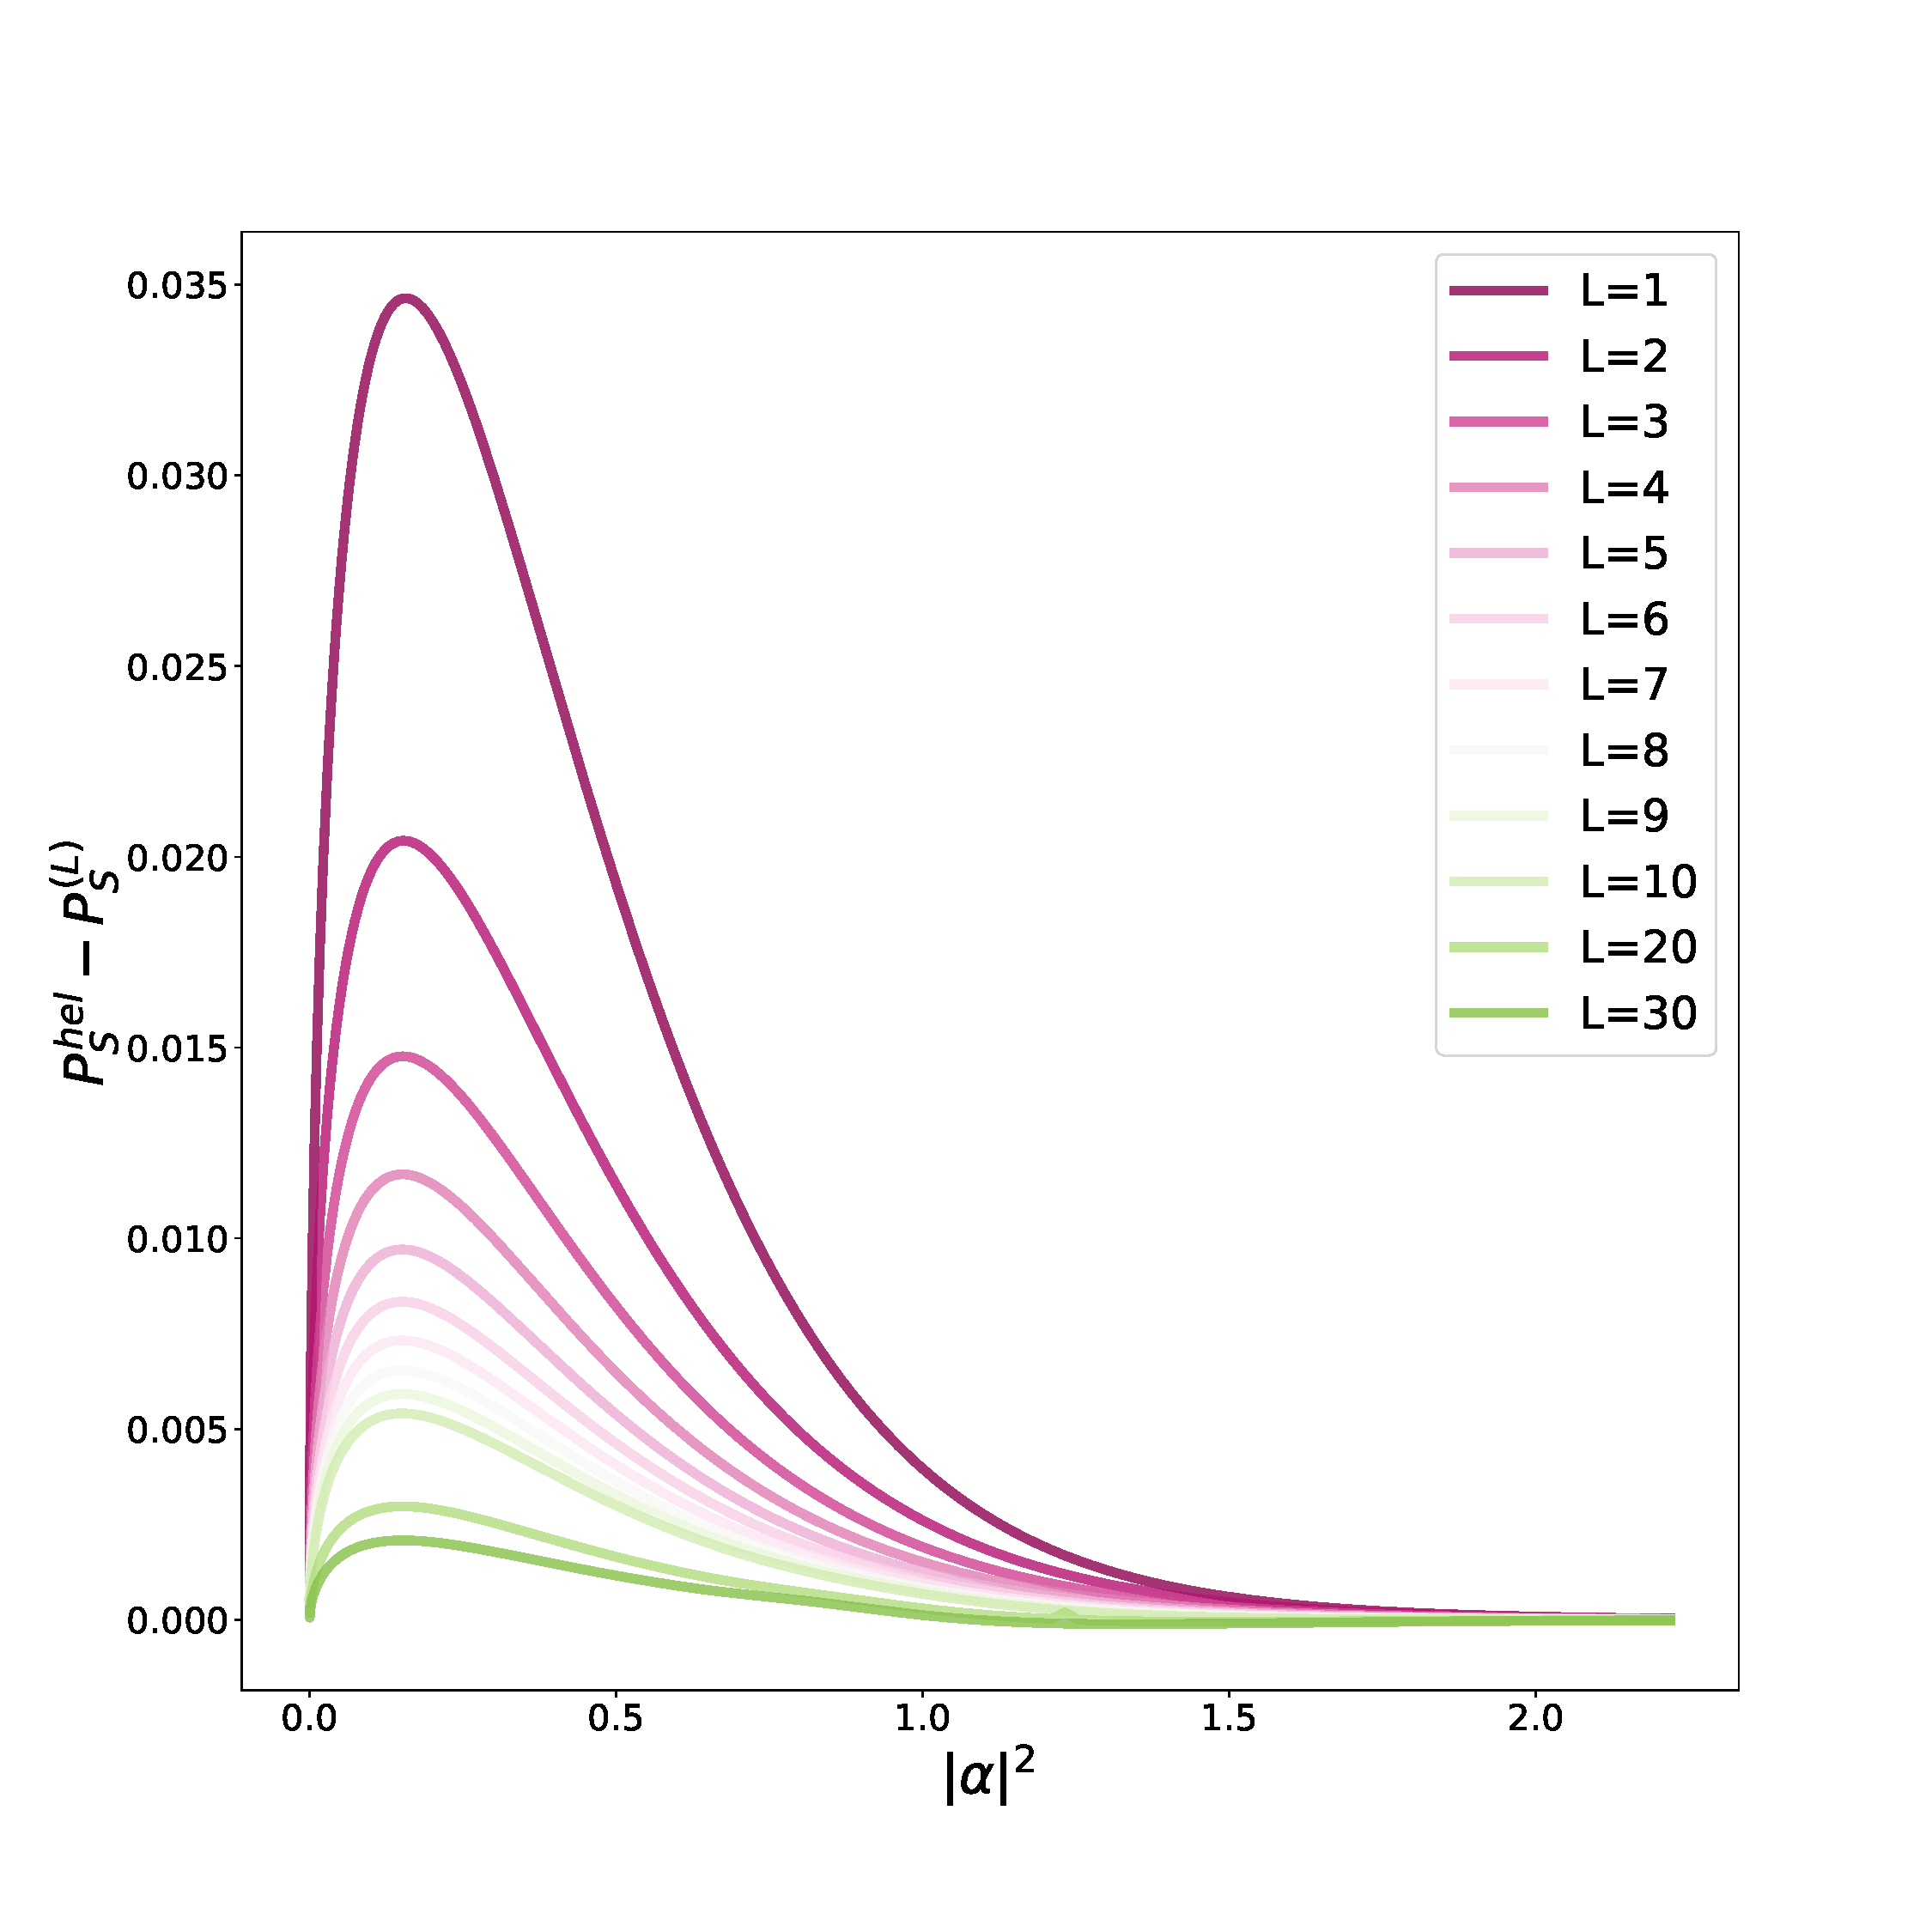
\includegraphics[width=1.\textwidth]{Figures/314/34_dp_results.pdf}
        \caption{}
        \label{fig:dpre1}
    \end{subfigure}
    \begin{subfigure}[b]{0.49\textwidth}
        \centering
        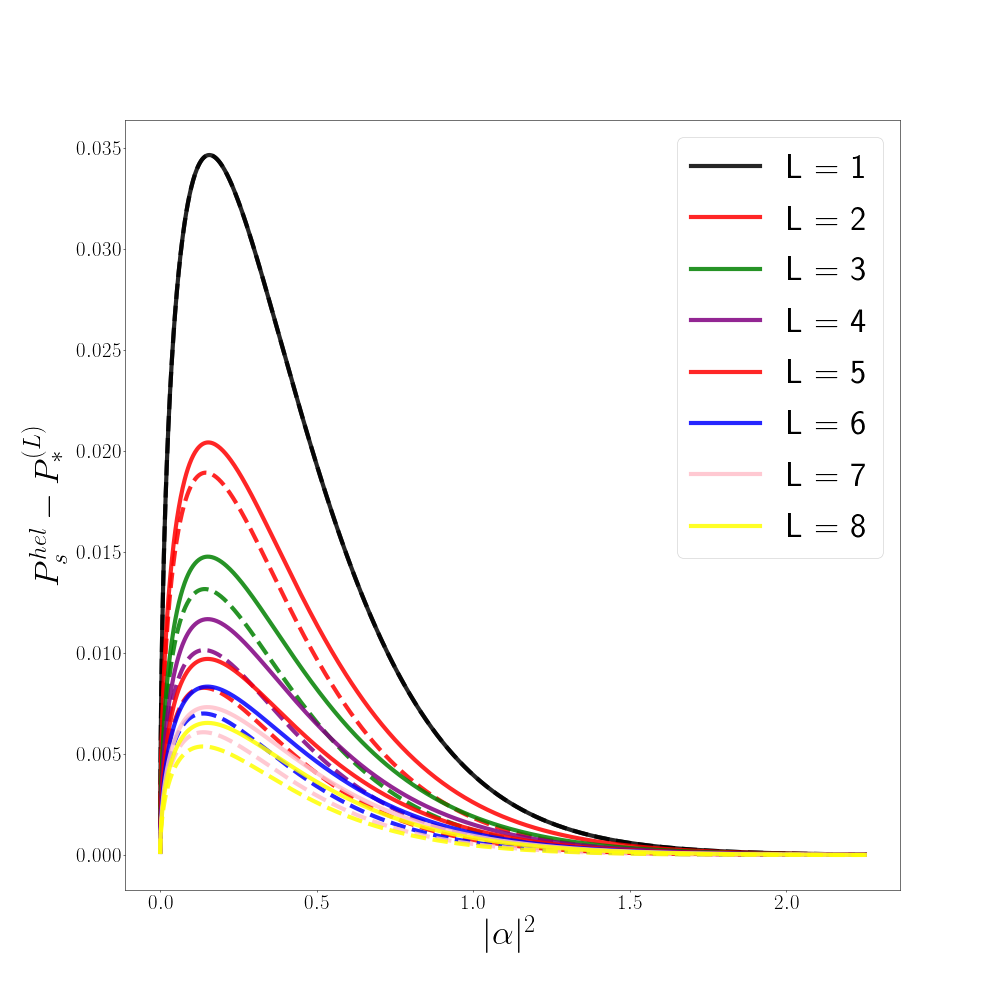
\includegraphics[width=1.\textwidth]{Figures/314/paper_dp_results_notation.png}
        \caption{}
        \label{fig:dpre2}
    \end{subfigure}
    \caption{We show the difference between the best probability of success attainable for a fix $L$ and the optimal probability of success in discriminating BPSK coherent states. The results were obtained by dynamic programming. \textit{Left panel}: the attenuations at the beam-splitters are fixed in such a way that each partial measurement deals with a state having the same intensity $\alpha^{\ell}_k=\frac{\alpha_k}{\sqrt{L-1}}$ for all $\ell$. \textit{Right panel}: we compare the advantage of adapting beam-splitter transmisivities as compared to the receivers considered in left panel and depicted in ~Fig.\ref{fig:dolinar_with_attas}.}
    \label{fig:dp_resu}
\end{figure}



\begin{figure}
\centering
  \begin{subfigure}[b]{.49\textwidth}
      \centering
      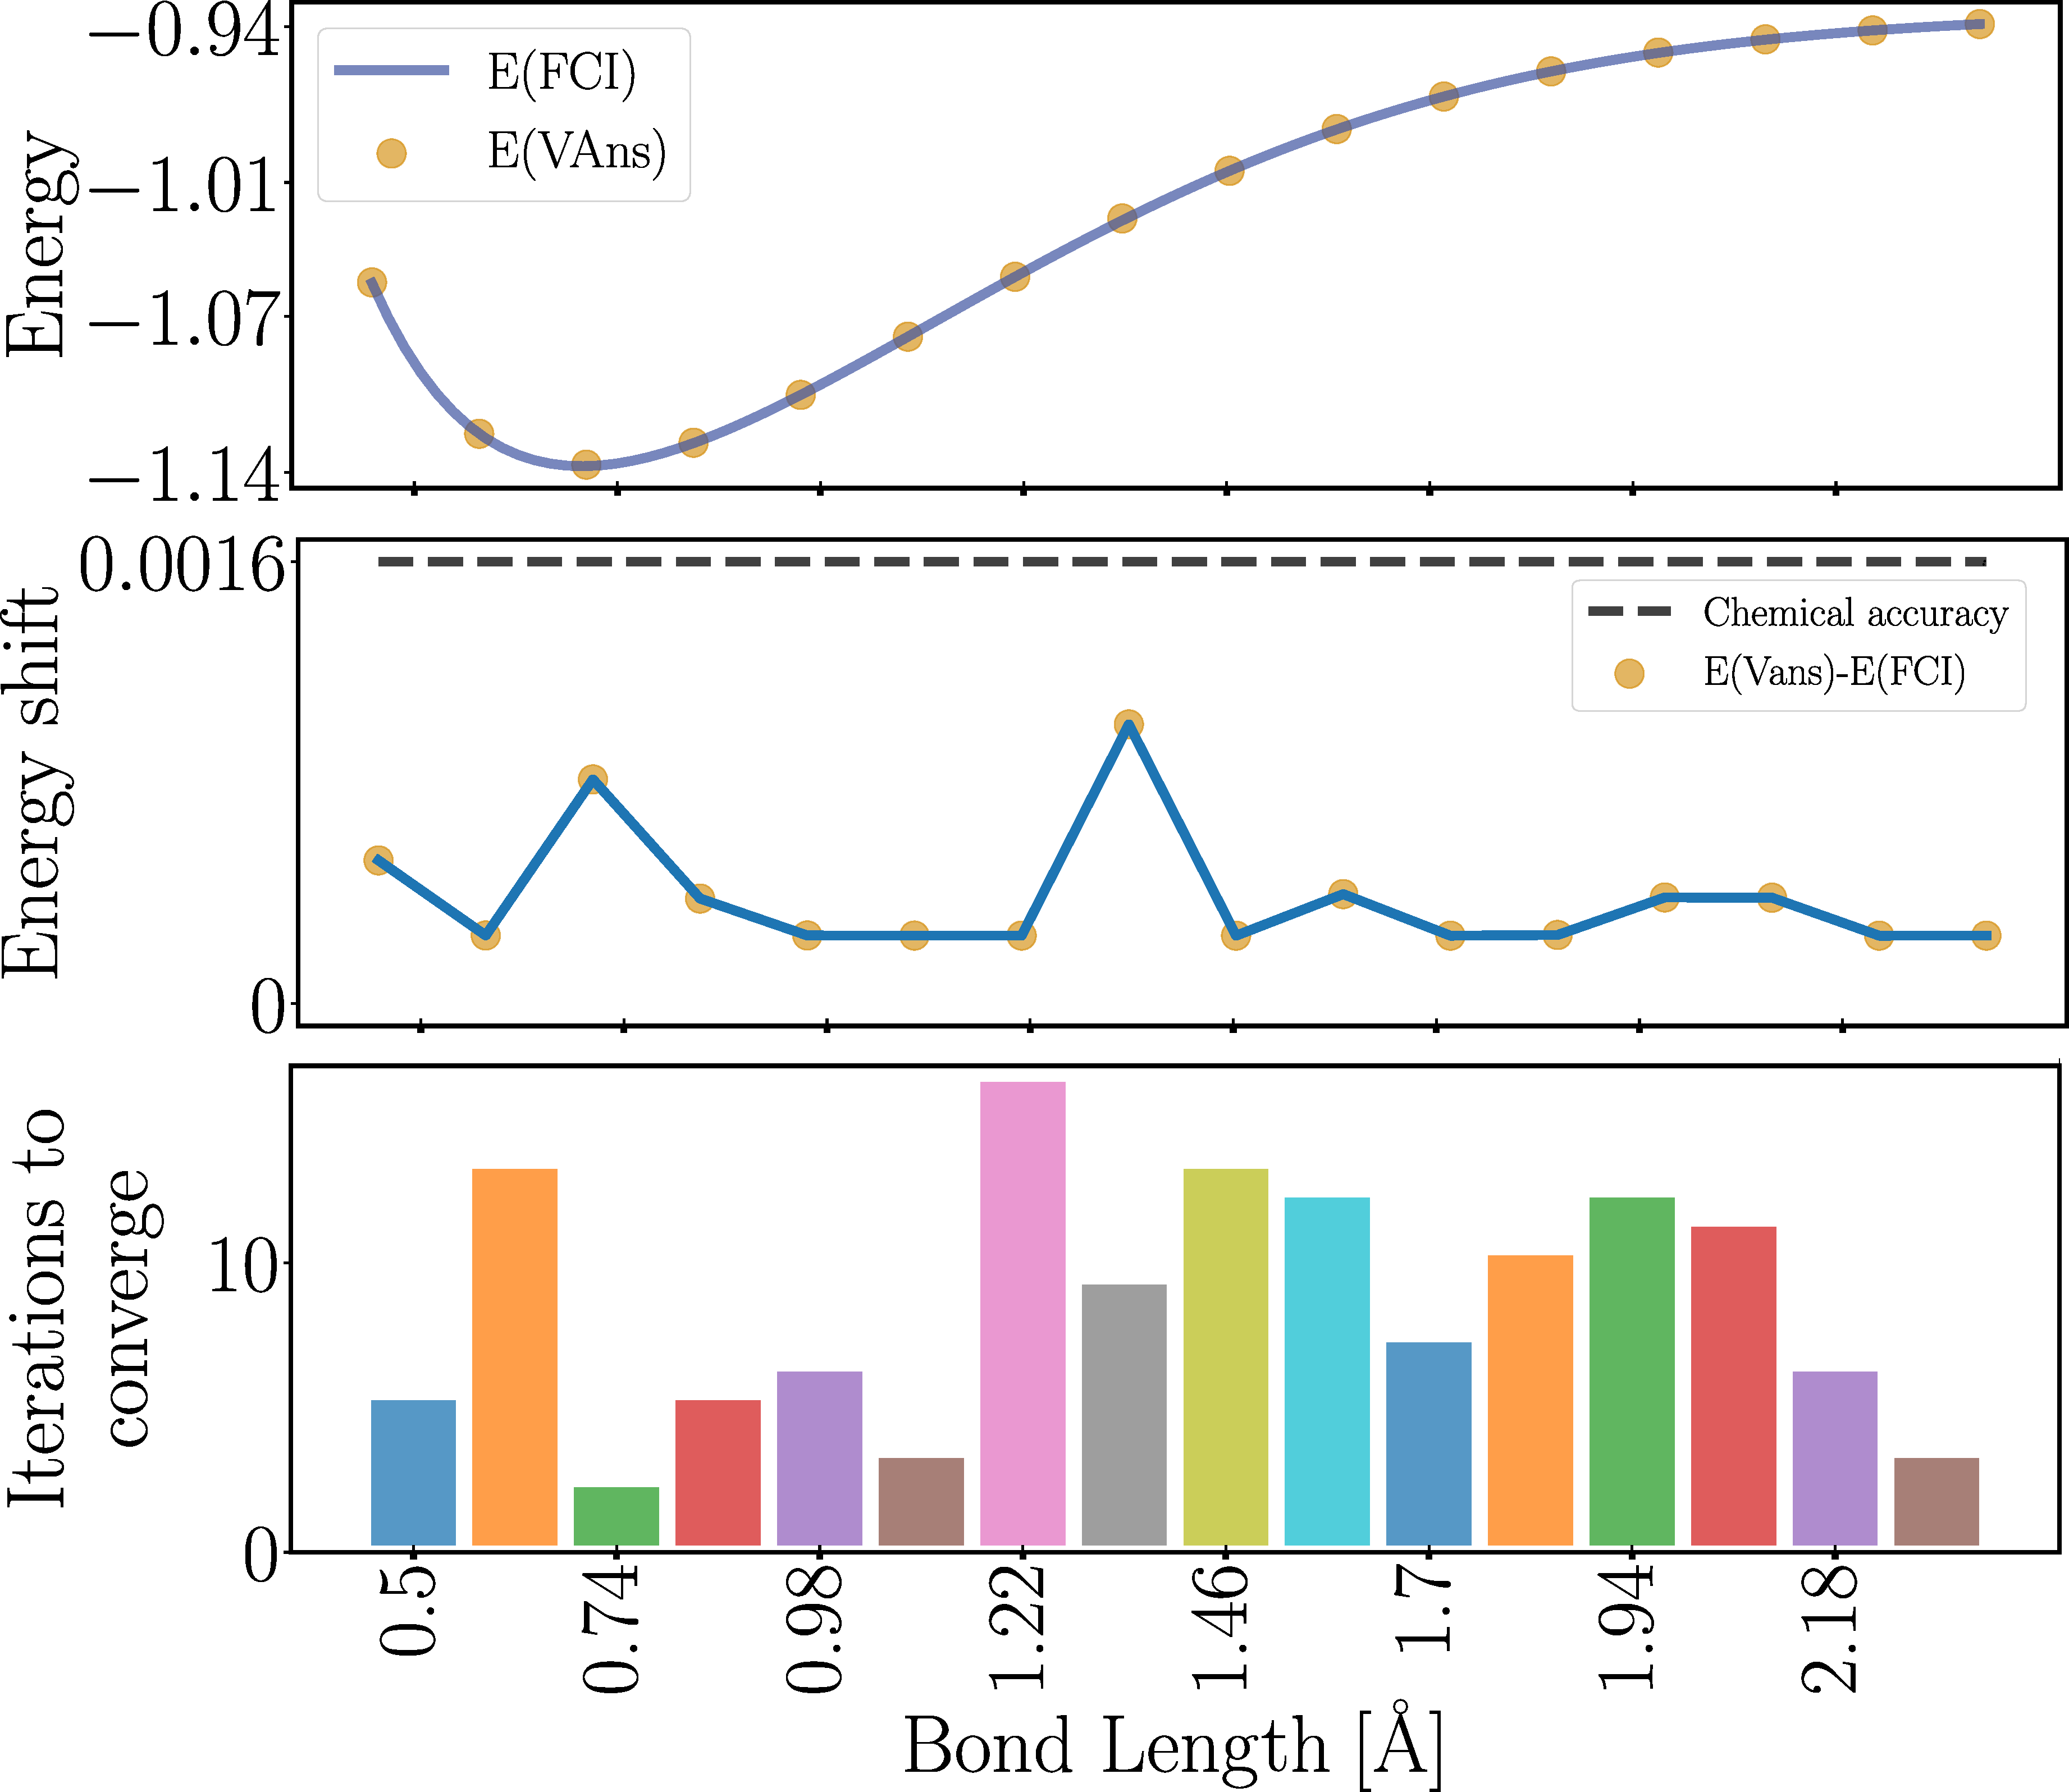
\includegraphics[width=1.\textwidth]{Figures/VANS/Fig9.pdf}
      \caption{x = y}
  \end{subfigure}
  \hfill
  \begin{subfigure}[b]{.49\textwidth}
      \centering
      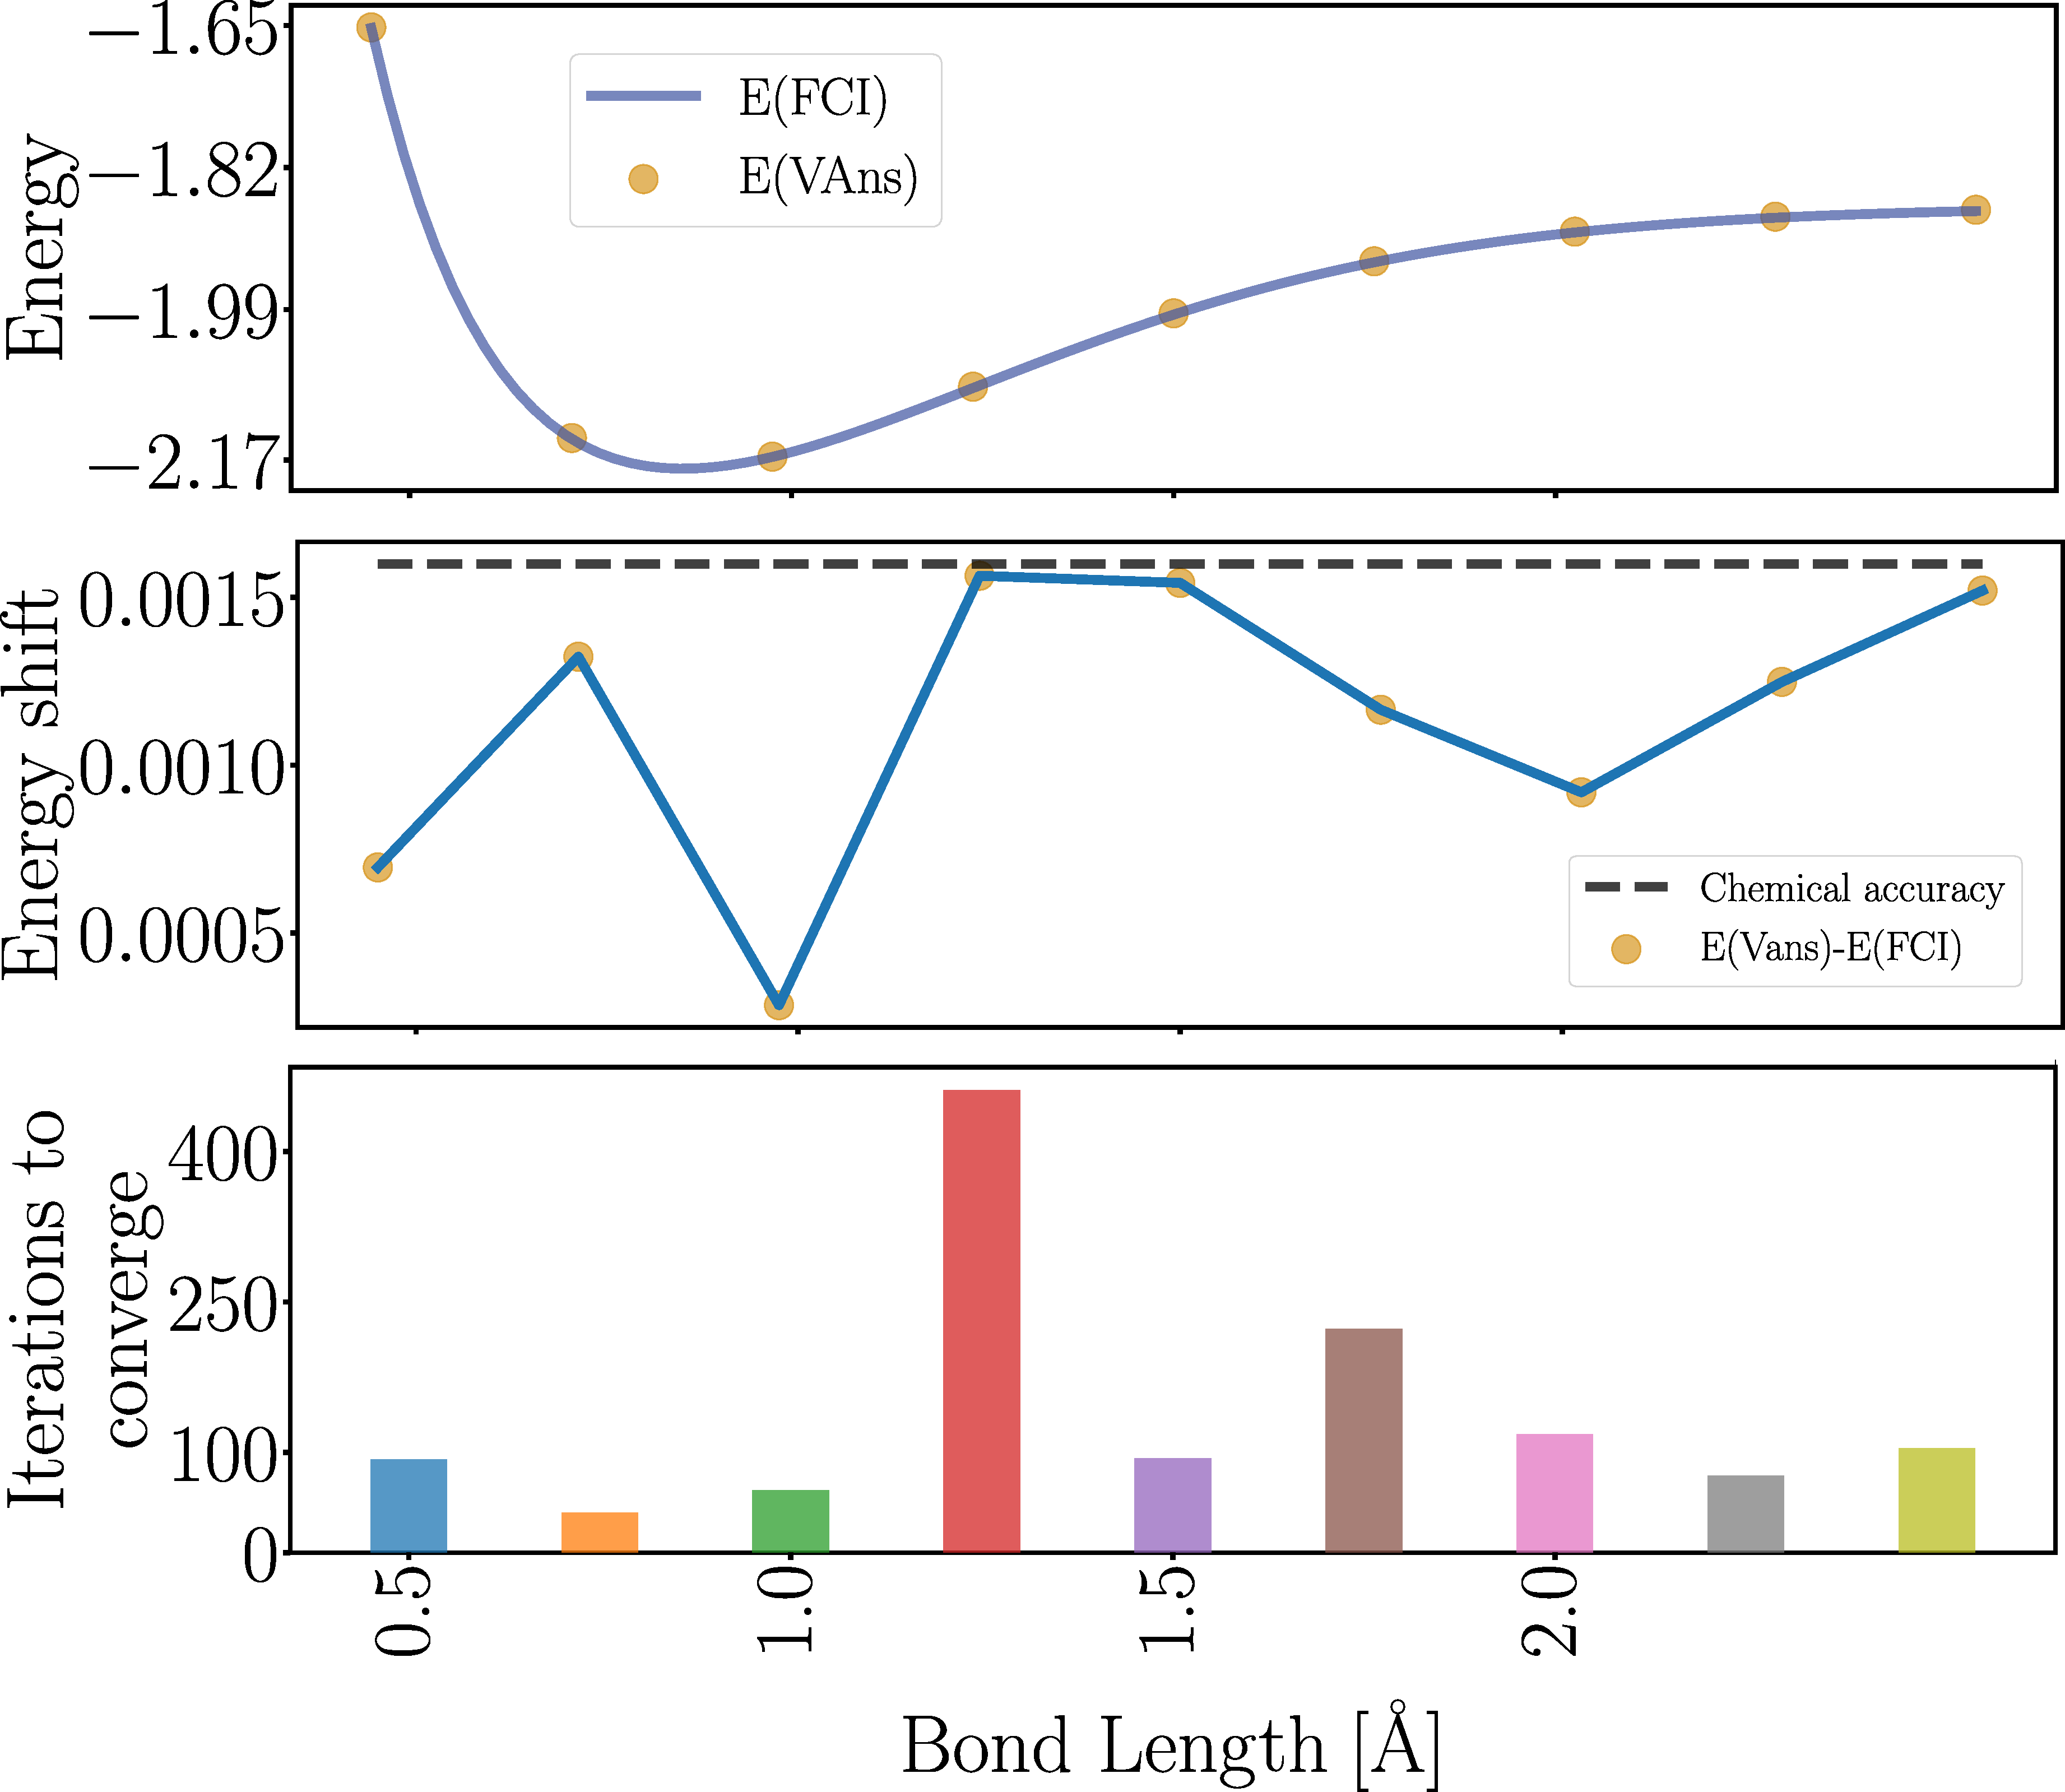
\includegraphics[width=1.\textwidth]{Figures/VANS/Fig12.pdf}
      \caption{x = y}
  \end{subfigure}
\caption{We show results of using VAns to obtain the ground state of a Hydrogen (H4) molecule, at different bond lengths. Here we use VAns in the VQE algorithm for the molecular Hamiltonian obtained after a Jordan-Wigner transformation, leading to a 4(8)-qubit circuit in left(right) panels. Top: Solid lines correspond to ground state energy as computed by the Full Configuration Interaction (FCI) method, whereas points correspond to energies obtained using VAns. Middle: Differences between exact and VAns ground state energies are shown. Dashed line corresponds to chemical accuracy, which stands for the ultimate accuracy experimentally reachable in such systems. Bottom: Number of iterations required by VAns until convergence are shown.}
\end{figure}


\begin{figure}
\centering
  \begin{subfigure}[b]{0.3\textwidth}
      \centering
      
\includegraphics[width=\textwidth]{Figures/giqlogo.png}
      \caption{x = y}
  \end{subfigure}
  \hfill
  \begin{subfigure}[b]{0.3\textwidth}
      \centering
      
\includegraphics[width=\textwidth]{Figures/giqlogo.png}
      \caption{x = y}
  \end{subfigure}
\caption{this is the big caption}
\end{figure}
